\documentclass{article}%
\usepackage[T1]{fontenc}%
\usepackage[utf8]{inputenc}%
\usepackage{lmodern}%
\usepackage{textcomp}%
\usepackage{lastpage}%
\usepackage[head=40pt,margin=0.5in,bottom=0.6in]{geometry}%
\usepackage{graphicx}%
%
\title{\textbf{Una misión de la oficina de Bachelet visitará Venezuela}}%
\author{YOSELIN GONZÁLEZ}%
\date{07/03/2019}%
%
\begin{document}%
\normalsize%
\maketitle%
\textbf{URL: }%
http://www.eluniversal.com/politica/34957/una{-}mision{-}de{-}la{-}oficina{-}de{-}bachelet{-}visitara{-}venezuela\newline%
%
\textbf{Periodico: }%
EU, %
ID: %
34957, %
Seccion: %
politica\newline%
%
\textbf{Palabras Claves: }%
NO\_TIENE\newline%
%
\textbf{Derecho: }%
2.1%
, Otros Derechos: %
\newline%
%
\textbf{\textit{El Consejo de los Derechos Humanos de la ONU retomará discusión sobre la situación en el país el 20 de marzo en la ONU con la presencia de la alta comisionada Michelle Bachelet}}%
\newline%
\newline%
%
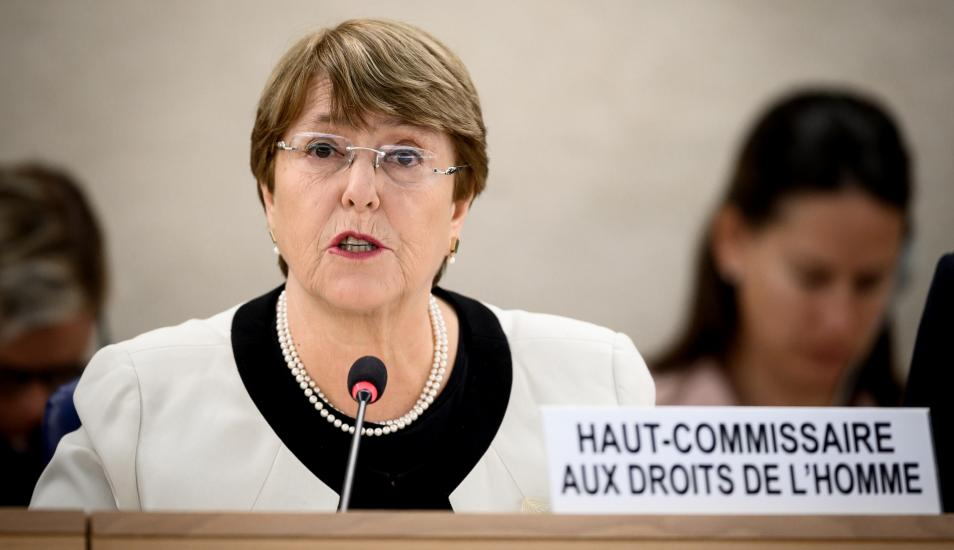
\includegraphics[width=300px]{EU_34957.jpeg}%
\newline%
%
Michelle Bachelet, la Alta Comisionada de los Derechos Humanos de la Organización de las Naciones Unidas (ONU), informó que enviará a una misión que trabaja para su oficina a visitar Venezuela el 10 de marzo para realizar una evaluación sobre la situación en el país, reseñó el portal web El Libero.%
\newline%
%
Detallan que el equipo estará integrado por cinco personas que permanecerán aproximadamente diez días, con la intención de visitar Caracas, Valencia, Barquisimeto y posiblemente Puerto Ordaz. Luego levantarán un informe sobre si existen las condiciones para un viaje de Bachelet.%
\newline%
%
Esperan verificar la existencia de una emergencia humanitaria compleja, abordar temas referidos a salud, alimentación, libertad de expresión, conflictividad social, vulneración de los derechos laborales y violación sistemática a los derechos humanos. Por esta razón se reunirán con la organización de la sociedad civil, víctimas y también con representantes de instituciones gubernamentales.  Se prevé que estén en el país hasta el 22 de marzo.%
\newline%
%
Dos personas de la sede en Ginebra, un oficial de la Oficina Regional para América del Sur del Alto Comisionado de Naciones Unidas para los Derechos Humanos (ACNUDH), con sede en Santiago de Chile, y otra persona de la sede en Panamá; además de un oficial de seguridad de las Naciones Unidas son los integrantes que conforman el grupo que visitará el Estado venezolano.%
\newline%
%
Por su parte, Bachelet indicó en un video posteado en su cuenta de Twitter que cuando la invitan a un país, se asegura de que puede desempeñar su papel como debería. "Que puedo ir y hablar con todo el mundo, de otro modo, sería inútil" dijo ante el Consejo de los Derechos Humanos de la ONU.%
\newline%
%
Explicó que sería un "fracaso" de su función si al visitar el país no puede reunirse con quien necesite. "Tengo que estar segura de que puedo realizar un informe completo, no uno sesgado" subrayó.%
\newline%
%
Además sostuvo que continuarán monitoreando la situación desde Panamá, en donde tienen un mandato del Consejo de los Derechos Humanos de la ONU, de igual forma, retomarán en profundidad la situación venezolana el próximo 20 de marzo, en presencia de la Alta Comisionada.%
\newline%
%
Presión internacional%
\newline%
%
En su alocución, Bachelet argumentó que la crisis política, económica y social por la que atraviesa Venezuela ha sido "exacerbada por sanciones" internacionales. La situación del país "ilustra claramente la manera en la que las violaciones de los derechos civiles y políticos {-}incluida la no defensa de las libertades fundamentales y la independencia de las instituciones clave{-} pueden acentuar un declive de los derechos económicos y sociales" agregó.%
\newline%
%
Asimismo, que esto demuestra que el rápido deterioro de esas condiciones económicas y sociales genera un mayor número de protestas, "una represión aún más grande y a nuevas violaciones de los derechos civiles y políticos".%
\newline%
%
A su juicio, esta todas esta situación se ha agravado por la presión internacional y que "la actual crisis política, económica, social e institucional resultante es alarmante".%
\newline%
%
El pasado 27 de febrero, durante un encuentro con la Ata Comisionada, el canciller Jorge Arreaza, reiteró la invitación oficial hecha en varias oportunidades por el mandatario Nicolás Maduro para recibirla en Venezuela.%
\newline%
%
Rusia critica sanciones%
\newline%
%
Por otra parte, el gobierno euroasiático considera que el endurecimiento de sanciones financieras por parte del gobierno estadounidense contra Venezuela, no facilitarán “una salida” a la situación económica que vive la nación.%
\newline%
%
Alexander Schetinin, director del Departamento de América Latina del Ministerio de Asuntos Exteriores de Rusia, dijo a Sputnik que “El recrudecimiento de la asfixia económica y financiera a la que recurre Estados Unidos, de ninguna manera, contribuirá a atenuar la situación en la que se encuentran la economía venezolana y la esfera social debido a esas sanciones”.%
\newline%
%
Además señaló que la ayuda humanitaria que EEUU intenta ingresar a territorio venezolano "no compensará los daños causados por las sanciones estadounidenses". Apuntó que la misma debería "despolitizada, imparcial y neutral", así como contribuir a mejorar la calidad de vida de los ciudadanos y no a conseguir “intereses mezquinos” de diferentes sectores políticos de la nación.%
\newline%
%
Rusia, es uno de los aliados del gobierno de Nicolás Maduro y en varias oportunidades ha rechazado las sanciones impuestas y las “acciones injerencistas” por parte de Norteamérica.%
\newline%
%
\end{document}